\section{\uppercase{Best views estimation}}\label{sec:best-views-estimation}

\noindent Implementation text.

\subsection{Reference surface point cloud}

\begin{itemize}
	\item The first step in the processing pipeline includes the generation of the multi-object reference point cloud that is assembled using the CAD data and the objects poses given by the simulator, which is later on filtered with a voxel grid algorithm to perform a regular spatial partition and extract the points that are in the surface voxels centroids
\end{itemize}
\begin{figure}
	\centering
	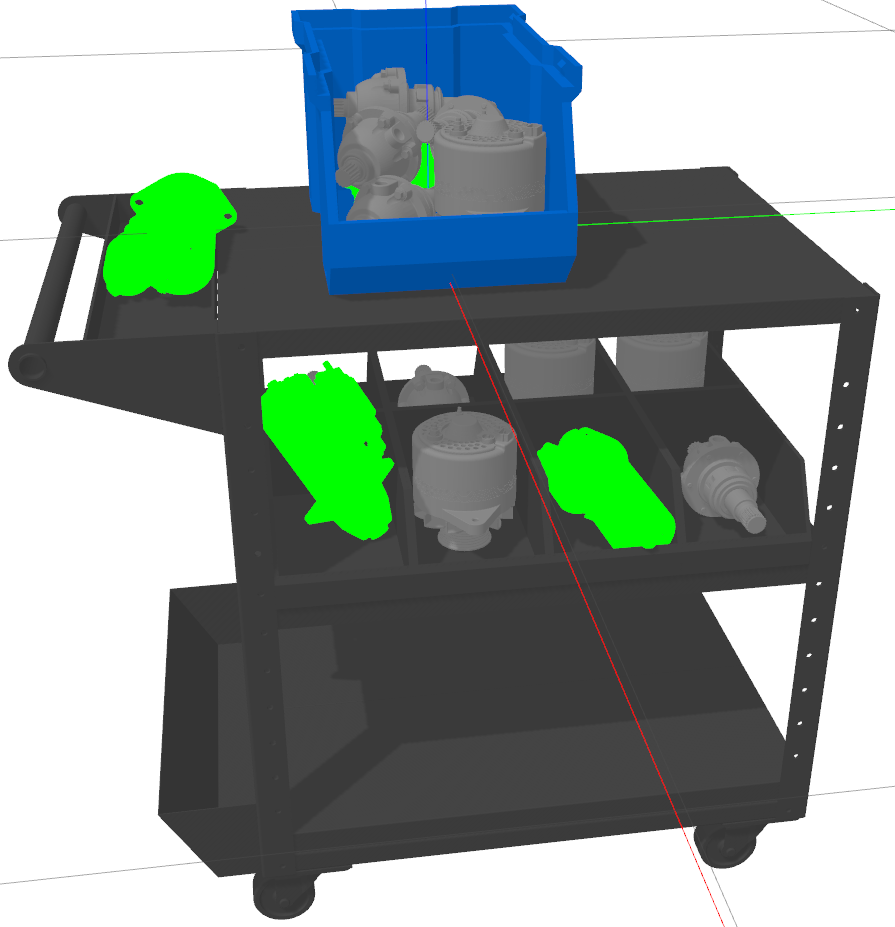
\includegraphics[height=.14\textheight]{sensor-data-processing/multimodel-environment}\hspace{2em}
	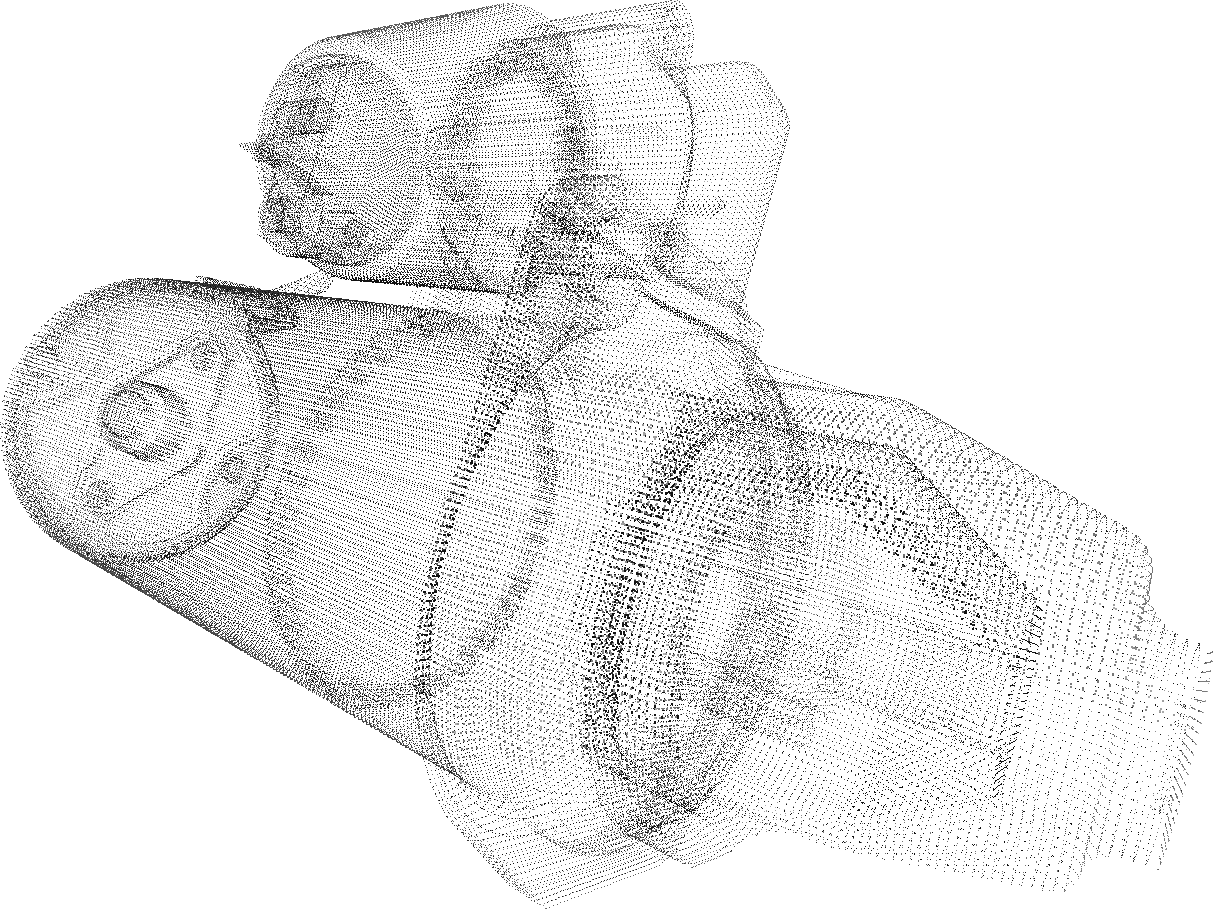
\includegraphics[height=.1\textheight]{sensor-data-processing/cad-model-pointcloud}
	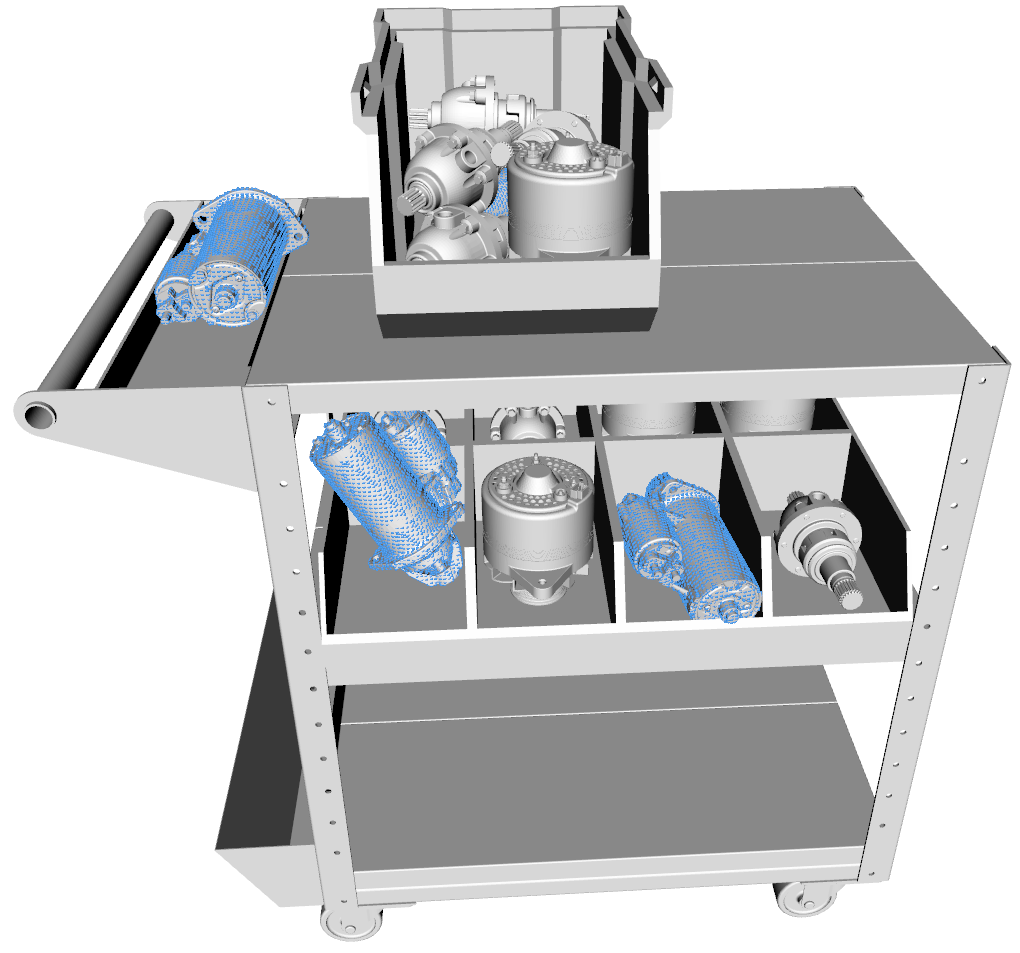
\includegraphics[height=.14\textheight]{sensor-data-processing/multimodel-pointclouds-with-cad}\hspace{2em}
	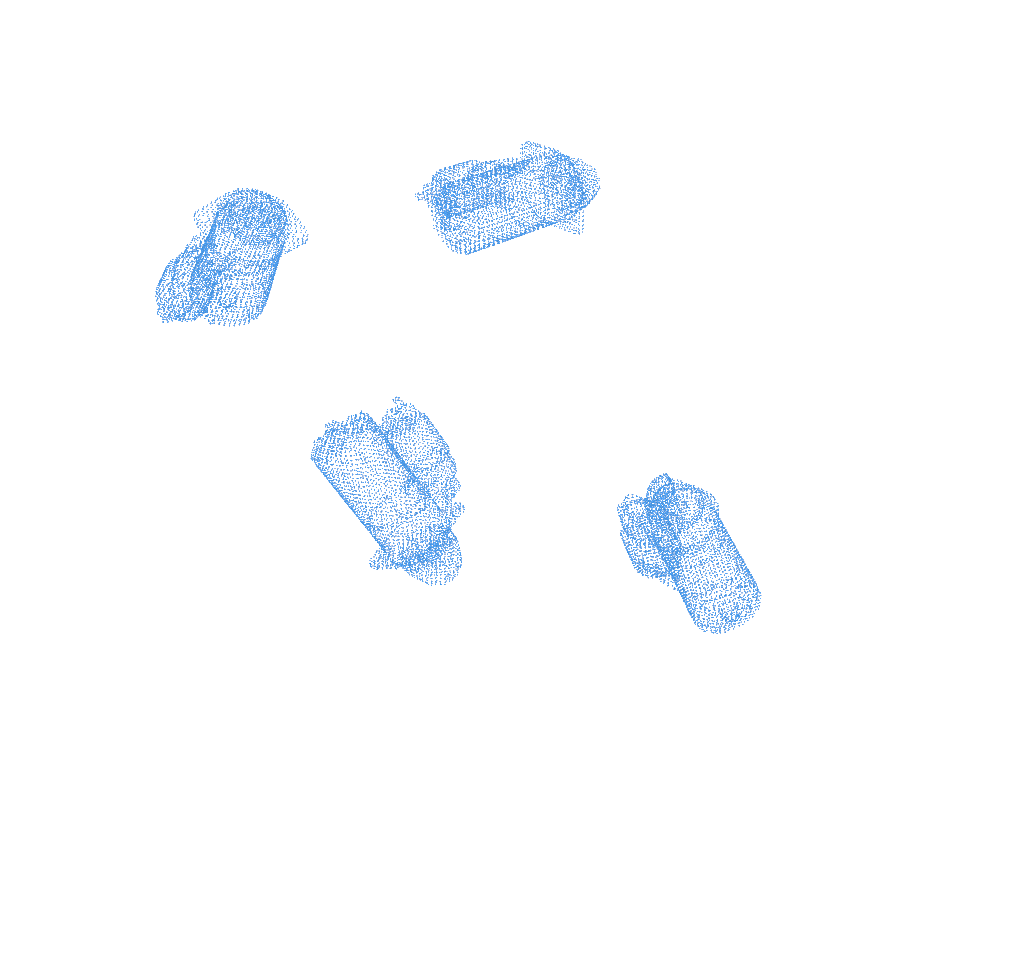
\includegraphics[height=.14\textheight]{sensor-data-processing/multimodel-pointclouds}
	\caption{The first image illustrates the color scene rendering in Gazebo with the target objects in green while the third and fourth images display the reference point cloud that was generated from the CAD points data shown on the second image}
\end{figure}


\subsection{Sensors data analysis}

\begin{itemize}
	\item Given a set of deployed sensors in the simulation world, for each sensor it is computed the voxelized point cloud of the observed target object(s) points:
	\begin{itemize}
		\item Color segmentation is performed to identify the sensor image pixels that belong to the target object(s) (which have a unique pure green material)
		\item For each image pixel associated with a target object, the 3D depth point is computed from the z-buffer depth image using the pinhole camera model
		\item The generated point cloud is transformed from the sensor into the world coordinate system frame
		\begin{itemize}
			\item Allows fast merging of point clouds generated from different sensors
		\end{itemize}
		\item A voxel grid filtering algorithm is applied to perform a regular space partition in which the points centroid are computed for each voxel
		\begin{itemize}
			\item Critical for allowing consistent evaluation of the object(s) observed surface area coverage percentage, even when the sensors have different resolution and are at different distances from the target object(s)
		\end{itemize}
	\end{itemize}
\end{itemize}

\begin{figure}
	\centering
	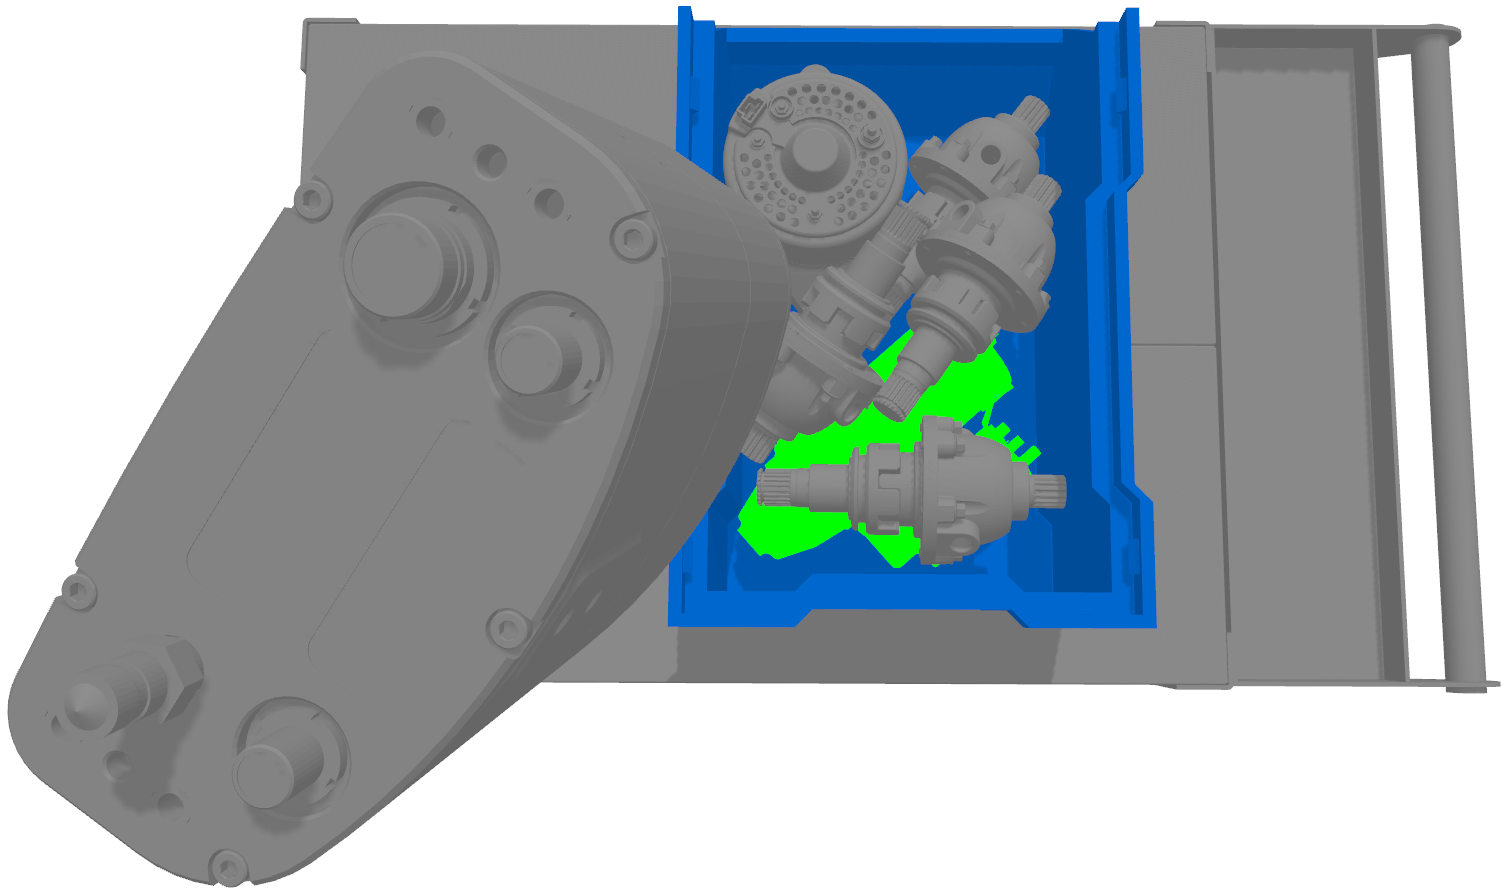
\includegraphics[height=.132\textheight]{sensor-data-processing/sensors-best-view}\\
	\vspace{0.5em}
	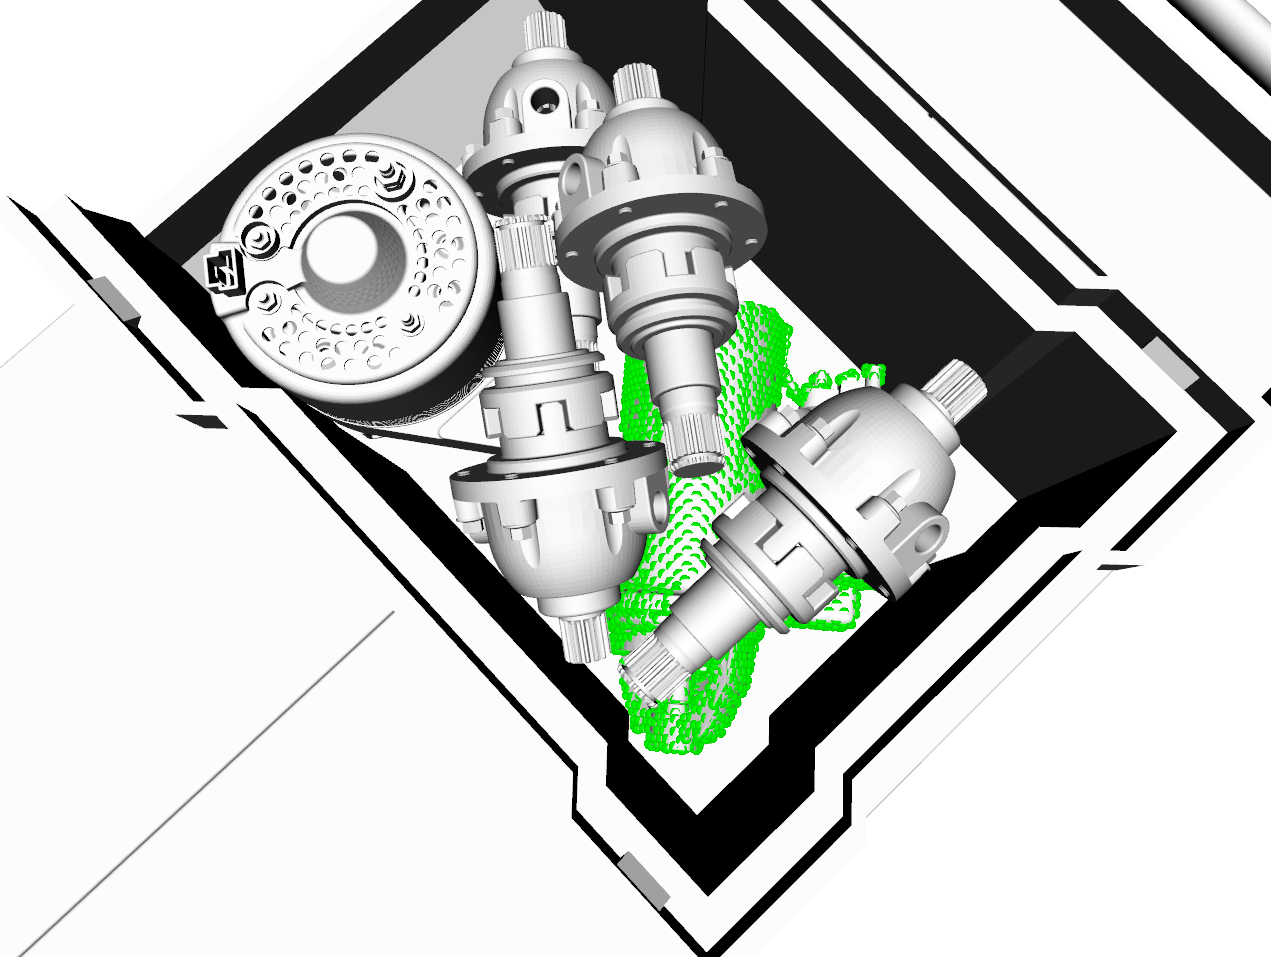
\includegraphics[height=.132\textheight]{sensor-data-processing/rviz-sensor-view}\hspace{2em}
	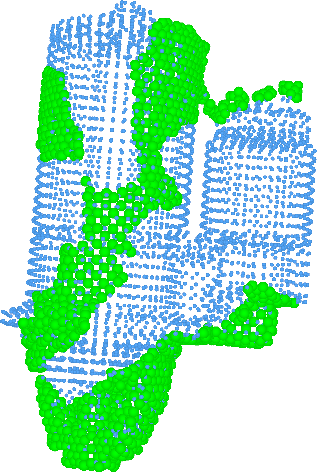
\includegraphics[height=.132\textheight]{sensor-data-processing/rviz-sensor-view-without-cad-with-model}
	\caption{Color image rendered with the Gazebo simulator (top image containing the scene and sensor) along with the generated point cloud for the target object taking into consideration the environment occlusions (bottom images, in which the green spheres are the observed points and the blue spheres are from the point cloud of the associated CAD model)}
\end{figure}


\subsection{Estimation of the best sensor}

After having the processed point cloud for each deployed sensor:
\begin{itemize}
	\item If only one sensor is enough (decision made by the system user):
	\begin{itemize}
		\item The surface coverage percentage for each sensor is computed
		\begin{itemize}
			\item Given that both the reference point cloud and the sensor data were filtered with a voxel grid with the same resolution and in the same coordinate system frame, calculating the surface coverage percentage can be efficiently computed by simply dividing the number of surface voxel points in the sensor data by the number of surface voxel points in the reference point cloud
		\end{itemize}
			\item The sensor that can observe the most surface area percentage of the target object(s) is chosen
	\end{itemize}
\end{itemize}


\subsection{Estimation of the best N sensors disposition}

After having the processed point cloud for each deployed sensor:
\begin{itemize}
	\item If several sensors can be used (decision made by the system user):
	\begin{itemize}
		\item Using a Random Sample Consensus (RANSAC) approach, a set of N sensors is chosen randomly
		\item The sensor data from the selected sensors is merged
		\item The voxel grid filter algorithm is applied to ensure that there is only one point per voxel
		\item The observable surface area percentage for the selected sensors is computed
		\item If the current subset of sensors achieved better observable surface area percentage than the current best, then it becomes the current best views estimation for the sensor disposition
		\item At the end of a given number of iterations or if the observable surface area percentage reaches a given threshold, the search is terminated, returning the best sensor disposition found
	\end{itemize}
\end{itemize}
